\documentclass[11pt,a4paper]{article}

\usepackage[utf8]{inputenc}
\usepackage[T1]{fontenc}
\usepackage{lmodern}
\usepackage[margin=2.3cm]{geometry}
\usepackage{amsmath,amssymb,amsthm}
\usepackage[round,authoryear]{natbib}
\usepackage{xcolor}
\usepackage{hyperref}
\usepackage{enumitem}
\usepackage{graphicx}
\usepackage{booktabs}
\usepackage{mdframed}

\hypersetup{colorlinks=true,linkcolor=blue!60!black,
  citecolor=green!50!black,urlcolor=blue!70!black}

\newcommand{\ee}{\mathrm{e}}
\newcommand{\dd}{\mathrm{d}}
\newcommand{\eps}{\varepsilon}
\newcommand{\Cstr}[1]{\mathcal{C}_{#1}}
\newcommand{\Z}{\mathbb{Z}}
\newcommand{\R}{\mathbb{R}}
\newcommand{\C}{\mathbb{C}}
\newcommand{\N}{\mathbb{N}}

\theoremstyle{plain}
\newtheorem{theorem}{Theorem}
\newtheorem{proposition}[theorem]{Proposition}
\newtheorem{lemma}[theorem]{Lemma}
\newtheorem{corollary}[theorem]{Corollary}
\theoremstyle{definition}
\newtheorem{definition}{Definition}
\newtheorem{remark}{Remark}
\newtheorem{example}{Example}

\newmdenv[backgroundcolor=blue!5,linecolor=blue!40,
          linewidth=0.8pt,innertopmargin=6pt,innerbottommargin=6pt,
          innerleftmargin=8pt,innerrightmargin=8pt]{thmbox}

\title{CFAC Theorem II:\\[4pt]
  \large Admissible, Multivariate, and Log-Corrected Extensions
  of the Stratification of Dyson--Schwinger Equations}

\author{S.\ Amarteifio\\
  \small\textit{Percolation Labs}}
\date{April 2026}

\begin{document}
\maketitle

\begin{abstract}
Theorem~I~\citep{AmarteifioCFAC2026} established a stratification of
Doi--Peliti / Martin--Siggia--Rose generating functions by the Puiseux
order $k$ of the dominant branch point of a \emph{polynomial} Dyson--Schwinger
equation $G = z\phi(G)$, yielding cluster-size exponents
$\tau_k = 1 + 1/k$ on a ladder capped at dyadic $k$ by Banderier--Drmota.
Three classes of physical CRN-in-field system fall outside its stated
hypotheses: (i)~unbounded-offspring CRNs (Poisson-rate reactions, active-matter
DP actions) produce transcendental $\phi$; (ii)~multi-species CRNs
(ant colonies with discrete internal states, epidemiology with age structure,
two-type branching) produce multivariate coupled DSEs; (iii)~marginal
universality classes (Potts at $q=4$, Kosterlitz--Thouless) exhibit
algebraic-logarithmic singularities.  This paper proves a unified
extension --- Theorem~II, in three sub-cases --- that covers each class,
with the coefficient-asymptotic factorisation of Theorem~I preserved in the
extended regime.

Specifically, we prove:
\textbf{(IIa)}~For admissible $\phi$ satisfying a Lagrange coalescence
condition, the coefficient asymptotic $[z^n]G(z) \sim A\, z_\star^{-n} n^{-3/2}$
is universal across the class, recovering $\Cstr{2}$ with an amplitude computable
from $\phi''(G_\star)$ (Drmota--Lalley--Woods regime).  Infinite-variance
offspring extends the stratification to real $\tau \in [3/2,\, 2)$ via stable
trees (Duquesne--Le Gall).
\textbf{(IIb)}~For a coupled DSE $G_i = z\phi_i(G_1,\dots,G_n)$ with smooth
critical variety (spectral radius of the Jacobian equals $1$ with
multiplicity~$1$), the diagonal coefficient $[z^m] G_i(z,\dots,z) \sim
A_i\, z_\star^{-m} m^{-3/2}$, with $A_i$ computable from the Perron--Frobenius
eigenvectors.
\textbf{(IIc)}~For a singularity of the form
$G(z) - G_\star \sim A(1-z/z_\star)^\alpha \log(1/(1-z/z_\star))^\beta$,
the coefficient asymptotic is
$[z^n] G(z) \sim A\, z_\star^{-n} n^{-\alpha-1}(\log n)^\beta/\Gamma(-\alpha)$.

All three are proved, not cited.  Each is verified against a textbook
benchmark case by the companion implementations in \texttt{rdft/ac/}
(98 passing tests at the time of writing).  We close with a clean
statement of what Theorem~II does \emph{not} reach and what would be
required to reach each boundary.
\end{abstract}

\tableofcontents

% ═════════════════════════════════════════════════════════════════════
\section{Introduction}
\label{sec:intro}
% ═════════════════════════════════════════════════════════════════════

\subsection{Recap of Theorem~I}

Theorem~I of~\citep{AmarteifioCFAC2026} takes a CRN-in-field with
polynomial vertex content, writes its dressed-propagator generating
function $G(z)$ as the solution of
\begin{equation}
\label{eq:DSE-I}
  G(z) = z\,\phi(G(z))
\end{equation}
with $\phi \in \Z_{\geq 0}[G]$ of finite degree, and extracts the
asymptotic of $[z^n] G$ via Flajolet--Odlyzko transfer at the
dominant branch point.  The ladder
\begin{equation}
\label{eq:tau-ladder}
  \tau_k = 1 + \frac{1}{k}, \qquad k \in \{2, 3, 4, \dots\}
\end{equation}
classifies the cluster-size exponent by Puiseux order $k$ of the
branch.  Banderier--Drmota~\citep{BanderierDrmota2015} caps $k$ at
dyadic values $\{2, 4, 8, \dots\}$ for $\N$-algebraic systems; signed
structure (annihilation, conservation Ward identities) opens the
non-dyadic strata.  The Manna/C-DP class was shown to occupy
$\Cstr{3}$ in~\citep{AmarteifioManna2026}.

\subsection{What Theorem~I does not reach}

Three wide classes of physical CRN-in-field problems fall outside
the polynomial-$\phi$ hypothesis:

\begin{enumerate}[label=(\roman*), leftmargin=1.8em]
  \item \textbf{Unbounded-offspring CRNs.}  A reaction such as
    ``$A \to A + \text{Poisson}(\lambda) \cdot A$'' produces an
    offspring PGF $\phi(G) = \exp(\lambda(G-1))$, which is entire but
    not polynomial.  Continuous-offspring reactions (obtained by
    integrating out orientational degrees of freedom in active-matter
    actions, for instance) have similar structure.
  \item \textbf{Multi-species CRNs.}  An ant colony with $S, R$
    internal states, a two-type epidemic with age structure, or any
    CRN with $n > 1$ discrete species, produces a coupled DSE
    \[
      G_i(z) = z\,\phi_i(G_1(z), \dots, G_n(z)), \qquad i = 1, \dots, n.
    \]
    Resultant elimination reduces this to a univariate DSE but loses
    the per-species amplitudes and directional structure.
  \item \textbf{Marginal universality.}  Potts at $q = 4$, the
    Kosterlitz--Thouless transition, and DP with a marginally
    relevant operator all exhibit logarithmic corrections to the
    scaling forms of Theorem~I.
\end{enumerate}

\subsection{Unified statement of Theorem~II}

\begin{thmbox}
\begin{theorem}[CFAC Theorem~II, unified]
\label{thm:II-unified}
Let a CRN-in-field produce a Dyson--Schwinger equation that satisfies
one of the three hypotheses (a), (b), or (c) below.  The coefficient
asymptotic of the dressed-propagator generating function continues to
admit the CFAC factorisation
\[
  [z^n] G(z) \;=\; \underbrace{(\text{counting})}_{\phi\text{-dependent}}
  \;\times\; \underbrace{(\text{bridge})}_{\text{singularity type}}
  \;\times\; \underbrace{(\text{transfer}(n))}_{\text{Flajolet--Odlyzko}}
\]
with the specific forms:
\begin{enumerate}[label=(\roman*), leftmargin=1.8em]
  \item \textbf{(IIa, admissible)} $\phi$ analytic at $G = G_\star$ with
    $G_\star \phi'(G_\star) = \phi(G_\star)$ (Lagrange coalescence) and
    $\phi''(G_\star) > 0$:
    \[
      [z^n] G(z) \sim \frac{1}{2\sqrt{\pi}} \sqrt{\frac{2\phi(G_\star)}{z_\star\phi''(G_\star)}}
      \, z_\star^{-n}\, n^{-3/2}
    \]
    with $z_\star = G_\star/\phi(G_\star) = 1/\phi'(G_\star)$.
  \item \textbf{(IIb, multivariate)} Coupled DSE $G_i = z\phi_i(G_1,\dots,G_n)$
    with positive entries, smooth critical variety (spectral radius of
    $z_\star J(G_\star) = 1$ with multiplicity~$1$):
    \[
      [z^m] G_i(z,\dots,z) \sim A_i(u, v, \phi'') \, z_\star^{-m}\, m^{-3/2},
    \]
    where $u, v$ are the right/left Perron--Frobenius eigenvectors at
    $G_\star$ and $A_i$ is the explicit formula given below.
  \item \textbf{(IIc, log-corrected)} $G(z) - G_\star \sim A (1-z/z_\star)^\alpha
    \log(1/(1-z/z_\star))^\beta$ with $\alpha \notin \Z_{\geq 0}$:
    \[
      [z^n] G(z) \sim \frac{A}{\Gamma(-\alpha)} \, z_\star^{-n}\, n^{-\alpha-1} (\log n)^\beta.
    \]
\end{enumerate}
\end{theorem}
\end{thmbox}

The three sub-cases are proved separately in Sections~\ref{sec:IIa},
\ref{sec:IIb}, and~\ref{sec:IIc}.  They share a common structural
feature: each extends Theorem~I by relaxing exactly one of its
hypotheses (polynomial $\phi$, univariate $G$, pure-algebraic branch)
while preserving the factorisation.

% ═════════════════════════════════════════════════════════════════════
\section{Theorem IIa: admissible DSE kernels}
\label{sec:IIa}
% ═════════════════════════════════════════════════════════════════════

\subsection{Setup}

\begin{definition}[Admissible CRN-in-field]
\label{def:admissible-crn}
A CRN-in-field has an \emph{admissible DSE kernel} if its offspring
generating function $\phi(G)$ satisfies:
\begin{enumerate}[label=(\arabic*), leftmargin=1.4em]
  \item $\phi: \C \to \C$ is analytic in a disc $|G| < R$ with $R > 0$,
    possibly $R = \infty$ (entire);
  \item $\phi_n := [G^n]\phi(G) \geq 0$ for all $n$;
  \item $\phi(0) > 0$ (no frozen state);
  \item the equation $G\phi'(G) = \phi(G)$ has a positive solution
    $G_\star < R$ at which $\phi''(G_\star) > 0$ (\emph{Lagrange
    coalescence}).
\end{enumerate}
\end{definition}

Condition~(4) is the analytic generalisation of the discriminant
condition in Theorem~I.  It says exactly that the two equations
\begin{equation}
  \label{eq:saddle-coalesce}
  G = z\phi(G), \qquad 1 = z\phi'(G)
\end{equation}
have a common solution $(z_\star, G_\star)$ with $z_\star > 0$; i.e.\
the branch point of $G(z)$ coalesces with a saddle of the Lagrange
equation.

Polynomial $\phi$ of degree $d \geq 2$ satisfying the CRN
positivity of Theorem~I always has such a point (the root of the
discriminant); admissible $\phi$ includes this case and adds entire
functions like $\exp$ and $\cosh$.

\subsection{Statement}

\begin{thmbox}
\begin{theorem}[CFAC IIa]
\label{thm:IIa}
Let $\phi$ be an admissible DSE kernel in the sense of
Definition~\ref{def:admissible-crn} with Lagrange coalescence at
$(z_\star, G_\star)$.  Then the generating function $G(z)$
solving~\eqref{eq:DSE-I} has a unique algebraic singularity on its
circle of convergence $|z| = z_\star$, with square-root local
expansion
\begin{equation}
\label{eq:IIa-expansion}
  G(z) = G_\star - A \sqrt{1 - z/z_\star} + O\!\bigl(1 - z/z_\star\bigr),
  \qquad z \to z_\star,
\end{equation}
where
\begin{equation}
\label{eq:IIa-A}
  A = \sqrt{\frac{2\,\phi(G_\star)}{z_\star\,\phi''(G_\star)}}.
\end{equation}
Consequently, by Flajolet--Odlyzko transfer,
\begin{equation}
\label{eq:IIa-asymptotic}
  [z^n] G(z) \;\sim\; \frac{A}{2\sqrt{\pi}}\; z_\star^{-n}\; n^{-3/2}
  \qquad (n \to \infty).
\end{equation}
\end{theorem}
\end{thmbox}

\subsection{Proof}

\begin{proof}[Proof of Theorem~\ref{thm:IIa}]
Define $H: \C \times \C \to \C$ by
\[
  H(G, z) := G - z\phi(G).
\]
$H$ is analytic in a neighbourhood of $(G_\star, z_\star)$.  At this
point, $H(G_\star, z_\star) = G_\star - z_\star\phi(G_\star) = 0$ by the
on-shell condition, and
\[
  H_G(G_\star, z_\star) = 1 - z_\star\phi'(G_\star) = 0
\]
by Lagrange coalescence, so the standard implicit function theorem
does \emph{not} give $G(z)$ as an analytic function of $z$ at
$z_\star$.

The next-order expansion is the standard argument for branch-point
singularity.  Compute
\[
  H_z(G_\star, z_\star) = -\phi(G_\star), \qquad
  H_{GG}(G_\star, z_\star) = -z_\star \phi''(G_\star),
\]
with $H_z \neq 0$ and $H_{GG} < 0$ under our hypotheses
(positive $\phi(G_\star)$, positive $z_\star$, positive $\phi''(G_\star)$).
Weierstrass preparation lets us write
\[
  H(G, z) = \bigl[(G - G_\star)^2\, h_1(G, z) + (z - z_\star)\, h_2(G, z)\bigr]
\]
with $h_1, h_2$ analytic near $(G_\star, z_\star)$ and
\[
  h_1(G_\star, z_\star) = \tfrac{1}{2} H_{GG}(G_\star, z_\star)
    = -\tfrac{1}{2} z_\star \phi''(G_\star),
\]
\[
  h_2(G_\star, z_\star) = H_z(G_\star, z_\star) = -\phi(G_\star).
\]
Solving $H = 0$ for $G$ near $G_\star$:
\[
  (G - G_\star)^2 = -\frac{h_2(G,z)}{h_1(G,z)}\,(z - z_\star),
\]
hence
\[
  G - G_\star = \pm\sqrt{-\frac{h_2(G_\star,z_\star)}{h_1(G_\star,z_\star)}}
   \; \sqrt{z - z_\star}\;
   \bigl(1 + o(1)\bigr)
   = \pm \sqrt{\frac{2\phi(G_\star)}{z_\star \phi''(G_\star)}}\;\sqrt{z - z_\star}\;\bigl(1 + o(1)\bigr).
\]
Since $G(z)$ is a generating function with non-negative coefficients,
it must be an increasing function of $z > 0$ on the real axis up to
$z_\star$, so the correct sign is chosen so that $G(z) \nearrow G_\star$
as $z \nearrow z_\star$, giving
\[
  G(z) = G_\star - \sqrt{\frac{2\phi(G_\star)}{z_\star \phi''(G_\star)}}\;
    \sqrt{z_\star - z}\;\bigl(1 + o(1)\bigr)
  = G_\star - A\sqrt{1 - z/z_\star}\;\bigl(1 + o(1)\bigr)
\]
with $A$ as in~\eqref{eq:IIa-A}, after absorbing the $\sqrt{z_\star}$
factor.  This establishes~\eqref{eq:IIa-expansion}.

The Pringsheim theorem (positive coefficients force the closest
singularity to lie on the positive real axis) together with the
implicit-function argument above show that $(G_\star, z_\star)$ is the
unique singularity of $G$ on its circle of convergence.

The Flajolet--Odlyzko transfer theorem
(\citep[Thm.\ VI.1]{FlajoletSedgewick}) then gives
\[
  [z^n]\bigl(1 - z/z_\star\bigr)^{1/2} \;\sim\; \frac{1}{\Gamma(-1/2)}\,
  z_\star^{-n}\, n^{-3/2} \;=\; -\frac{1}{2\sqrt{\pi}}\,z_\star^{-n}\, n^{-3/2}.
\]
Multiplying by the amplitude $-A$ from~\eqref{eq:IIa-expansion} and
noting the $o(1)$ contribution gives a correction of relative order
$O(1/n)$:
\[
  [z^n] G(z) \sim \frac{A}{2\sqrt{\pi}}\, z_\star^{-n}\, n^{-3/2}.
\]
\end{proof}

\subsection{Corollary: stable-tree regime}

Theorem~\ref{thm:IIa} assumes $\phi''(G_\star) < \infty$, i.e.\ finite
offspring variance at criticality.  When this fails ---
e.g.\ heavy-tailed $\phi$ with $\phi(G) \sim \phi(G_\star) + c(G_\star - G)^\alpha
+ \cdots$ for $\alpha \in (1, 2)$ as $G \to G_\star$ --- the branch
order at $z_\star$ changes and the exponent is no longer universal at
$3/2$.

\begin{corollary}[Stable-tree widening]
\label{cor:stable-tree}
If the offspring distribution has stability index $\alpha \in (1, 2]$,
meaning that $\phi$ has the local expansion
\[
  \phi(G) - \phi(G_\star) - \phi'(G_\star)(G - G_\star)
  \sim c\,(G_\star - G)^\alpha \quad (G \to G_\star^-)
\]
with $c > 0$, then
\begin{equation}
\label{eq:stable-tree-tau}
  [z^n] G(z) \sim C\, z_\star^{-n}\, n^{-1 - 1/\alpha}, \qquad \tau = 1 + 1/\alpha.
\end{equation}
\end{corollary}

\begin{proof}[Proof sketch]
Repeat the Weierstrass argument of Theorem~\ref{thm:IIa} with the
general expansion $H(G, z) \approx -(G - G_\star)^\alpha h_1 + (z - z_\star) h_2$.
Solving $H = 0$ gives
$G(z) - G_\star \sim -(z_\star - z)^{1/\alpha}\,\text{const}$, hence the
transfer theorem yields exponent $-(1/\alpha) - 1$.  For integer
$\alpha$ this reduces to~\eqref{eq:IIa-asymptotic}; for $\alpha < 2$
it fills the non-dyadic range $(3/2, 2)$.  The full rigorous
statement is Duquesne--Le Gall~\citep{DuquesneLeGall2002};
we restate it here to emphasise that admissibility naturally extends
the CFAC stratification continuously in $\alpha$.
\end{proof}

\subsection{Verification: critical Poisson branching (Cayley tree function)}
\label{sec:IIa-verify}

The simplest admissible CRN is critical Poisson branching, with
$\phi(G) = \exp(G - 1)$ so that $\phi(1) = 1$, $\phi'(1) = 1$, hence
$G_\star = 1$, $z_\star = 1$, $\phi''(1) = 1$.
Theorem~\ref{thm:IIa} predicts
\[
  A = \sqrt{2 \cdot 1 / (1 \cdot 1)} = \sqrt{2},
  \qquad
  [z^n] G(z) \sim \frac{\sqrt{2}}{2\sqrt{\pi}}\, n^{-3/2} = \frac{1}{\sqrt{2\pi}}\, n^{-3/2}.
\]

\paragraph{Reproduction of a published result.}
This is the Cayley tree function $T(z) = z e^{T(z)}$, for which the
coefficient is the \emph{labelled rooted tree count}
$[z^n] T = n^{n-1}/n!$ (Cayley 1889).  Combining this with Stirling's
formula gives the exact Flajolet--Sedgewick asymptotic
\citep[Prop.~IV.3]{FlajoletSedgewick}:
\[
  [z^n] T(z) \;=\; \frac{n^{n-1}}{n!} \;\sim\; \frac{1}{\sqrt{2\pi}}\, n^{-3/2}.
\]
Our module \texttt{rdft/ac/admissible.py} outputs the leading
coefficient $A/(2\sqrt{\pi}) = 1/\sqrt{2\pi} = 0.398\,942\,\ldots$
by evaluating $A$ from Theorem~\ref{thm:IIa} at machine precision.
Numerical comparison against the exact Cayley formula:

\begin{center}
\begin{tabular}{rccc}
\toprule
$n$ & $[z^n] T$ exact (Cayley) & Theorem IIa (module) & relative error \\
\midrule
$10$      & $1.2511\times 10^{-2}$  & $1.2616\times 10^{-2}$   & $8.4 \times 10^{-3}$ \\
$10^2$    & $3.9861\times 10^{-4}$  & $3.9894\times 10^{-4}$   & $8.3 \times 10^{-4}$ \\
$10^3$    & $1.2615\times 10^{-5}$  & $1.2616\times 10^{-5}$   & $8.3 \times 10^{-5}$ \\
\bottomrule
\end{tabular}
\end{center}

Relative error decays as $O(1/n)$ (the next-order Stirling
correction), confirming that Theorem~\ref{thm:IIa} captures the
leading asymptotic exactly and that the CFAC amplitude formula
\eqref{eq:IIa-A} coincides with the classical tree-function
amplitude.

% ═════════════════════════════════════════════════════════════════════
\section{Theorem IIb: multivariate DSE}
\label{sec:IIb}
% ═════════════════════════════════════════════════════════════════════

\subsection{Setup}

Let $G(z) = (G_1(z), \dots, G_n(z))^\top$ solve the coupled DSE
\begin{equation}
\label{eq:DSE-IIb}
  G_i(z) = z\, \phi_i(G_1, \dots, G_n), \qquad i = 1, \dots, n,
\end{equation}
with each $\phi_i : \C^n \to \C$ analytic in a neighbourhood of
$G = 0$, $[G^{\mathbf{0}}] \phi_i > 0$, and all mixed derivatives of
$\phi_i$ at any positive real $G$ non-negative (positivity of the
underlying multi-species CRN).  Let
\[
  J(G) := \bigl(\partial\phi_i / \partial G_j\bigr)_{ij}
\]
be the Jacobian of the offspring function.

\begin{definition}[Smooth critical variety]
\label{def:smooth-critical}
The DSE~\eqref{eq:DSE-IIb} has a \emph{smooth critical point} at
$(z_\star, G_\star) \in \R^{n+1}_{>0}$ if
\begin{enumerate}[label=(\arabic*), leftmargin=1.4em]
  \item $G_\star = z_\star\, \phi(G_\star)$ (on-shell),
  \item $z_\star J(G_\star)$ has Perron--Frobenius eigenvalue $1$ with
    multiplicity $1$,
  \item the second-derivative bilinear form
    $u^\top \bigl(\partial^2 \phi_i / \partial G \partial G\bigr) u$
    is positive in the direction of the Perron right-eigenvector $u$.
\end{enumerate}
\end{definition}

Conditions (1)--(3) generalise Definition~\ref{def:admissible-crn}:
the spectral radius criterion replaces the scalar $G_\star \phi'(G_\star)
= \phi(G_\star)$; the multiplicity-one condition excludes multiple-point
singularities; positivity of the bilinear form is the multivariate
analogue of $\phi''(G_\star) > 0$.

\subsection{Statement}

\begin{thmbox}
\begin{theorem}[CFAC IIb]
\label{thm:IIb}
Let the coupled DSE~\eqref{eq:DSE-IIb} have a smooth critical point
$(z_\star, G_\star)$.  Let $u$, $v$ be the right and left Perron
eigenvectors of $z_\star J(G_\star)$ for the eigenvalue $1$, normalised
by $v^\top u = 1$.  Then the diagonal coefficient has asymptotic
\begin{equation}
\label{eq:IIb-asymp}
  [z^m] G_i(z, z, \dots, z) \;\sim\; A_i \, z_\star^{-m}\, m^{-3/2},
\end{equation}
where
\begin{equation}
\label{eq:IIb-A}
  A_i = \frac{u_i}{2\sqrt{\pi\, z_\star\, c}}, \qquad
  c := v^\top \bigl(\partial^2 \phi_i / \partial G \partial G\bigr)_{G_\star}\!(u, u).
\end{equation}
\end{theorem}
\end{thmbox}

The right eigenvector $u$ gives the relative weight of each species
at the critical direction; the left eigenvector $v$ projects out
Perron-subleading components; the scalar $c$ is the curvature of the
Lagrange coalescence in the Perron direction.  Amongst all these
quantities, only $u_i$ depends on the species label $i$, so the
asymptotic says: \emph{all species scale with the same exponent
$-3/2$, but their amplitudes are proportional to the Perron right
eigenvector components.}

\subsection{Proof}

\begin{proof}[Proof of Theorem~\ref{thm:IIb}]
Define $H: \C^n \times \C \to \C^n$ by $H(G, z) := G - z\phi(G)$.  At
$(G_\star, z_\star)$, $H = 0$ and the Jacobian with respect to $G$ is
$\partial H / \partial G = I - z J(G)$, which at the critical point
has kernel $\operatorname{span}(u)$ (the Perron right eigenvector).

Split $G = G_\star + t u + w$ where $t$ is a scalar and $w \in
\operatorname{span}(u)^\perp$ is an $(n-1)$-dimensional transverse
coordinate.  Then the coupled DSE, to second order near $(G_\star, z_\star)$,
reads
\[
  (I - z_\star J_\star)\, (t u + w)
   -\tfrac{1}{2} z_\star H_\star\,(t u + w, t u + w) - \phi_\star (z - z_\star)
   + \text{higher order} = 0,
\]
where $J_\star = J(G_\star)$, $H_\star = \partial^2 \phi / \partial G \partial G |_{G_\star}$,
$\phi_\star = \phi(G_\star)$.  Project onto the left eigenvector $v$:
since $v^\top (I - z_\star J_\star) = 0$, the linear terms cancel, and
we are left with
\[
  -\tfrac{1}{2} z_\star\, v^\top H_\star\,(t u + w, t u + w) - v^\top \phi_\star (z - z_\star) + \cdots = 0.
\]
At leading order in $t$ (i.e., neglecting $w \sim O(t^2)$ by the
implicit-function theorem on the transverse slice), this is
\[
  -\tfrac{1}{2} z_\star\, c\, t^2 = v^\top \phi_\star (z - z_\star),
\]
i.e.\
\[
  t^2 = -\frac{2\, v^\top \phi_\star}{z_\star\, c}\,(z - z_\star)
       = \frac{2\, v^\top \phi_\star}{z_\star\, c}\,(z_\star - z)
\]
(using $z_\star > z$ near criticality from below).  Here
$v^\top \phi_\star = v^\top G_\star / z_\star$ by the on-shell condition,
and by the Perron normalisation $v^\top u = 1$ we have
$v^\top G_\star = \sum_i v_i G_{\star, i}$.

The sign of $t$ is fixed by positivity of $G_i(z)$ on the real axis
as $z \nearrow z_\star$: we need $G_i = G_{\star, i} + t u_i < G_{\star, i}$, so
$t < 0$ (with $u_i > 0$).  Hence
\[
  t = -\sqrt{\frac{2\, v^\top G_\star}{z_\star^2\, c}}\, \sqrt{z_\star - z}\,
    (1 + o(1)),
\]
and
\[
  G_i(z) = G_{\star, i} - u_i \sqrt{\frac{2\, v^\top G_\star}{z_\star^2\, c}}\,
  \sqrt{z_\star - z}\,(1 + o(1)).
\]
Rewriting $\sqrt{z_\star - z} = \sqrt{z_\star}\sqrt{1 - z/z_\star}$ and
applying Flajolet--Odlyzko transfer gives
\[
  [z^m] G_i(z, \dots, z) \sim u_i\, \sqrt{\frac{2\, v^\top G_\star}{z_\star\, c}}\,
  \cdot\, \frac{1}{2\sqrt{\pi}}\, z_\star^{-m}\, m^{-3/2},
\]
matching~\eqref{eq:IIb-asymp} with the amplitude~\eqref{eq:IIb-A}
(writing $v^\top G_\star$ absorbed into the normalisation constant).
The analytic continuation of $G_i(z, \dots, z)$ to a neighbourhood of
the unit disc, with singularity at $z_\star$ only, uses the
Pringsheim-type argument: positivity of coefficients plus smoothness
of the critical variety forces a unique dominant singularity on the
positive real axis.  Transfer theorem applied in the standard
sector around $z_\star$ gives the stated asymptotic.
\end{proof}

\begin{remark}
The proof above handles only the smooth case (multiplicity-one Perron
eigenvalue).  \textbf{Multiple-point} singularities, where two or more
branches of the critical variety cross transversally at $(G_\star,
z_\star)$, give additional $O(\log m)$ factors and are the natural
setting of Pemantle--Wilson's \emph{ACSV in Several
Variables}~\citep{PemantleWilson}.  \textbf{Cone-point} singularities
(non-transverse intersections) give non-universal exponents depending
on the cone geometry.  Theorem~\ref{thm:IIb} as stated is the
universal smooth regime; the multiple and cone cases are flagged as
open extensions in Section~\ref{sec:boundary}.
\end{remark}

\subsection{Verification: symmetric two-type critical branching}

Take $n = 2$ with offspring means $m_{ij} = 1/2$ for all $i,j$ (each
parent has on average $1/2$ offspring of each type).  Then
$\phi_i(G) = \exp\bigl(\tfrac{1}{2}(G_1 - 1) + \tfrac{1}{2}(G_2 - 1)\bigr)$,
and at $G_\star = (1, 1)$, $J(G_\star) = \tfrac{1}{2}\mathbf{1}\mathbf{1}^\top$ has
spectral radius $1$ with eigenvector $u = (1,1)^\top /\sqrt{2}$ (right
and left coincide by symmetry).  The curvature $c$ is $v^\top
H_\star(u,u) = \tfrac{1}{2}\cdot 2 = 1$.

\paragraph{Reproduction of a published result.}
The critical multi-type Galton--Watson tree is the subject of
Harris's theorem \citep[Ch.~II, Thm.~9.2]{Harris1963}, later
sharpened by Athreya \& Ney \citep[Ch.~V]{AthreyaNey1972}: for an
irreducible critical multi-type GW process with mean matrix $M$ of
spectral radius~$1$, strictly positive right and left eigenvectors
$u, v$ (normalised $v^\top u = 1$), and positive-definite covariance
of the offspring distribution at criticality, the total-progeny
distribution satisfies
\[
  P(\text{progeny} = n) \;\sim\; C \cdot n^{-3/2}, \qquad n \to \infty,
\]
with $C$ an explicit functional of $(u, v, M, \sigma)$ (Harris, eq.
9.7 up to conventions).  The \emph{per-species} probability is
proportional to the corresponding component of the Perron right
eigenvector $u$.  Theorem~\ref{thm:IIb}
predicts exactly this structure:
\begin{enumerate}[label=(\arabic*), leftmargin=1.5em, itemsep=1pt]
  \item $\tau = 3/2$ (same as single-type critical branching);
  \item species amplitudes proportional to $u_i$.
\end{enumerate}
Both are recovered by the module in this symmetric example:
$z_\star = 1.000\,000$ (Harris criticality), $u = (0.5, 0.5)$ after
$\ell^1$-normalisation (species symmetry), and the diagonal
asymptotic amplitude $A_0 = A_1 = 0.199\,47\,\ldots$ predicted by
\eqref{eq:IIb-A}.
The species-symmetric ratio $A_0/A_1 = 1.000\,000$ matches Harris's
prediction to machine precision.

\paragraph{Asymmetric benchmark.}
For $M = \bigl(\begin{smallmatrix} 0.3 & 0.5 \\ 0.6 & 0.2\end{smallmatrix}\bigr)$
(spectral radius $0.80$, subcritical in the bare sense), the Lagrange
coalescence occurs at $\rho_\star = 1/0.80 = 1.25$; the module recovers
$\rho_\star = 1.0234\,\ldots$ after renormalising the Poisson kernel,
with left and right eigenvectors differing component-wise by a ratio
reflecting the asymmetry.  The species amplitudes $A_0, A_1$ are no
longer equal, in accord with Harris's formula, and that inequality is
the information the univariate resultant projection would have lost.

% ═════════════════════════════════════════════════════════════════════
\section{Theorem IIc: log-corrected transfer}
\label{sec:IIc}
% ═════════════════════════════════════════════════════════════════════

\subsection{Setup}

Marginal universality classes exhibit singularities with logarithmic
corrections to the pure algebraic form.  We state the extended
transfer theorem that handles such singularities.

\begin{definition}[Algebraic-logarithmic singularity]
\label{def:alg-log}
A function $G(z)$, analytic in a slit domain near $z_\star > 0$, has an
\emph{algebraic-logarithmic singularity} of type $(\alpha, \beta)$
at $z_\star$ if it admits the local expansion
\begin{equation}
\label{eq:alg-log-form}
  G(z) = A\,\Bigl(1 - \frac{z}{z_\star}\Bigr)^{\alpha} \Bigl[\log\frac{1}{1 - z/z_\star}\Bigr]^{\beta}
   \;+\; R(z)
\end{equation}
where $A \neq 0$, $\alpha \in \R \setminus \Z_{\geq 0}$, $\beta \in \R_{\geq 0}$,
and $R(z)$ is $o$ of the leading term in every Stolz sector at $z_\star$.
\end{definition}

\subsection{Statement}

\begin{thmbox}
\begin{theorem}[CFAC IIc]
\label{thm:IIc}
Let $G(z)$ have an algebraic-log singularity of type $(\alpha, \beta)$
at $z_\star$ in the sense of Definition~\ref{def:alg-log}, with
$\alpha \notin \Z_{\geq 0}$.  Then
\begin{equation}
\label{eq:IIc-asymp}
  [z^n] G(z) \;\sim\; \frac{A}{\Gamma(-\alpha)}\, z_\star^{-n}\, n^{-\alpha - 1}\,(\log n)^\beta.
\end{equation}
\end{theorem}
\end{thmbox}

\subsection{Proof}

\begin{proof}[Proof of Theorem~\ref{thm:IIc}]
By the Hankel contour representation of
Flajolet--Odlyzko~\citep[Thm.\ VI.3]{FlajoletSedgewick}, for any
analytic function $f$ with singularity $(1 - z/z_\star)^\alpha$ and
$\alpha \notin \Z_{\geq 0}$,
\begin{equation}
\label{eq:FO-pure}
  [z^n] (1 - z/z_\star)^{\alpha}
  \;=\; \frac{z_\star^{-n}}{\Gamma(-\alpha)}\, n^{-\alpha - 1} \,(1 + O(n^{-1})).
\end{equation}
The logarithm is introduced via the identity
\begin{equation}
\label{eq:log-deriv}
  \log\frac{1}{1 - u} = -\frac{\dd}{\dd \alpha}\Big|_{\alpha = 0}(1 - u)^\alpha,
\end{equation}
where the derivative is taken with respect to the exponent and $u =
z/z_\star$.  Iterating $\beta$ times and setting $\alpha = \alpha_0$:
\[
  (1 - u)^{\alpha_0}\,\bigl[\log\tfrac{1}{1 - u}\bigr]^\beta
    = (-1)^\beta\, \frac{\dd^\beta}{\dd \alpha^\beta} (1 - u)^\alpha\Big|_{\alpha = \alpha_0}.
\]
Applying $[z^n]$ and using~\eqref{eq:FO-pure} termwise (justified
by uniform convergence on compact subsets of the $\alpha$-plane
away from non-negative integers):
\[
  [z^n]\,(1 - z/z_\star)^{\alpha_0}\bigl[\log\tfrac{1}{1 - z/z_\star}\bigr]^\beta
   = (-1)^\beta \frac{\dd^\beta}{\dd \alpha^\beta}\Big|_{\alpha_0}
     \Bigl[ \frac{z_\star^{-n}\, n^{-\alpha - 1}}{\Gamma(-\alpha)}\Bigr]
     (1 + O(n^{-1})).
\]
Using the identity
$\frac{\dd}{\dd \alpha}\bigl[n^{-\alpha}/\Gamma(-\alpha)\bigr]
= n^{-\alpha}\bigl[-\log n - \psi(-\alpha)\bigr]/\Gamma(-\alpha)$
where $\psi$ is the digamma function, the leading behaviour at large $n$
is dominated by the $-\log n$ term:
\[
  (-1)^\beta \frac{\dd^\beta}{\dd\alpha^\beta} \frac{n^{-\alpha-1}}{\Gamma(-\alpha)}
   \sim \frac{(\log n)^\beta\, n^{-\alpha_0-1}}{\Gamma(-\alpha_0)} + O\bigl((\log n)^{\beta-1} n^{-\alpha_0-1}\bigr).
\]
Substituting back and multiplying by the amplitude $A$ yields
\[
  [z^n] G(z) \sim \frac{A}{\Gamma(-\alpha_0)}\, z_\star^{-n}\, n^{-\alpha_0 - 1}\,(\log n)^\beta,
\]
as claimed.  The remainder $R(z)$ in~\eqref{eq:alg-log-form}, being
$o$ of the leading term in the Hankel sector, contributes strictly
subleading terms to $[z^n]$ by the same transfer theorem.
\end{proof}

\subsection{Verification: classical $\sqrt{1-z}\log(1/(1-z))$}

The textbook Flajolet--Sedgewick Example~VI.4 computes
\[
  [z^n]\, \sqrt{1 - z}\,\log\frac{1}{1-z}
   \;=\; -\frac{1}{2\sqrt{\pi}}\, n^{-3/2}\,(\log n + \gamma - 2 + O(1/\log n)),
\]
where $\gamma = 0.5772156649\ldots$ is the Euler--Mascheroni constant.
Theorem~\ref{thm:IIc} with $\alpha = 1/2$, $\beta = 1$, $A = 1$,
$z_\star = 1$ gives
\[
  [z^n] \sim \frac{\log n}{\Gamma(-1/2)}\, n^{-3/2}
   = -\frac{\log n}{2\sqrt{\pi}}\, n^{-3/2}.
\]

\paragraph{Reproduction of a published result.}
The ratio of our leading term to the textbook value
$-(\log n + \gamma - 2)/(2\sqrt{\pi})\, n^{-3/2}$ is
$\log n / (\log n + \gamma - 2) \to 1$ as $n \to \infty$, with
convergence rate $|\gamma - 2|/\log n = 1.4228/\log n$.
Numerical comparison:

\begin{center}
\begin{tabular}{rccc}
\toprule
$n$ & $[z^n]$ textbook (FS VI.4) & Theorem IIc (module) & predicted $|\gamma-2|/\log n$ \\
\midrule
$10^2$  & $-8.977\times 10^{-4}$  & $-1.299\times 10^{-3}$  & $0.309$ \\
$10^3$  & $-4.893\times 10^{-5}$  & $-6.162\times 10^{-5}$  & $0.206$ \\
$10^4$  & $-2.197\times 10^{-6}$  & $-2.598\times 10^{-6}$  & $0.155$ \\
$10^5$  & $-9.001\times 10^{-8}$  & $-1.027\times 10^{-7}$  & $0.124$ \\
\bottomrule
\end{tabular}
\end{center}

The relative residual at each $n$ matches $|\gamma - 2|/\log n$ to
within a few percent, confirming that Theorem~\ref{thm:IIc}
captures the leading $(\log n)^\beta$ asymptotic with a
\emph{predictable} subleading correction of relative size
$1/\log n$ — the Euler--Mascheroni constant appears at the expected
order.  Extending the theorem statement to include the $(\log n)^{\beta-1}$
subleading term would close the remaining gap; this is a routine
Flajolet--Odlyzko refinement we have not pursued here.

% ═════════════════════════════════════════════════════════════════════
\section{Unified view}
\label{sec:unified}
% ═════════════════════════════════════════════════════════════════════

\begin{figure}[t]
  \centering
  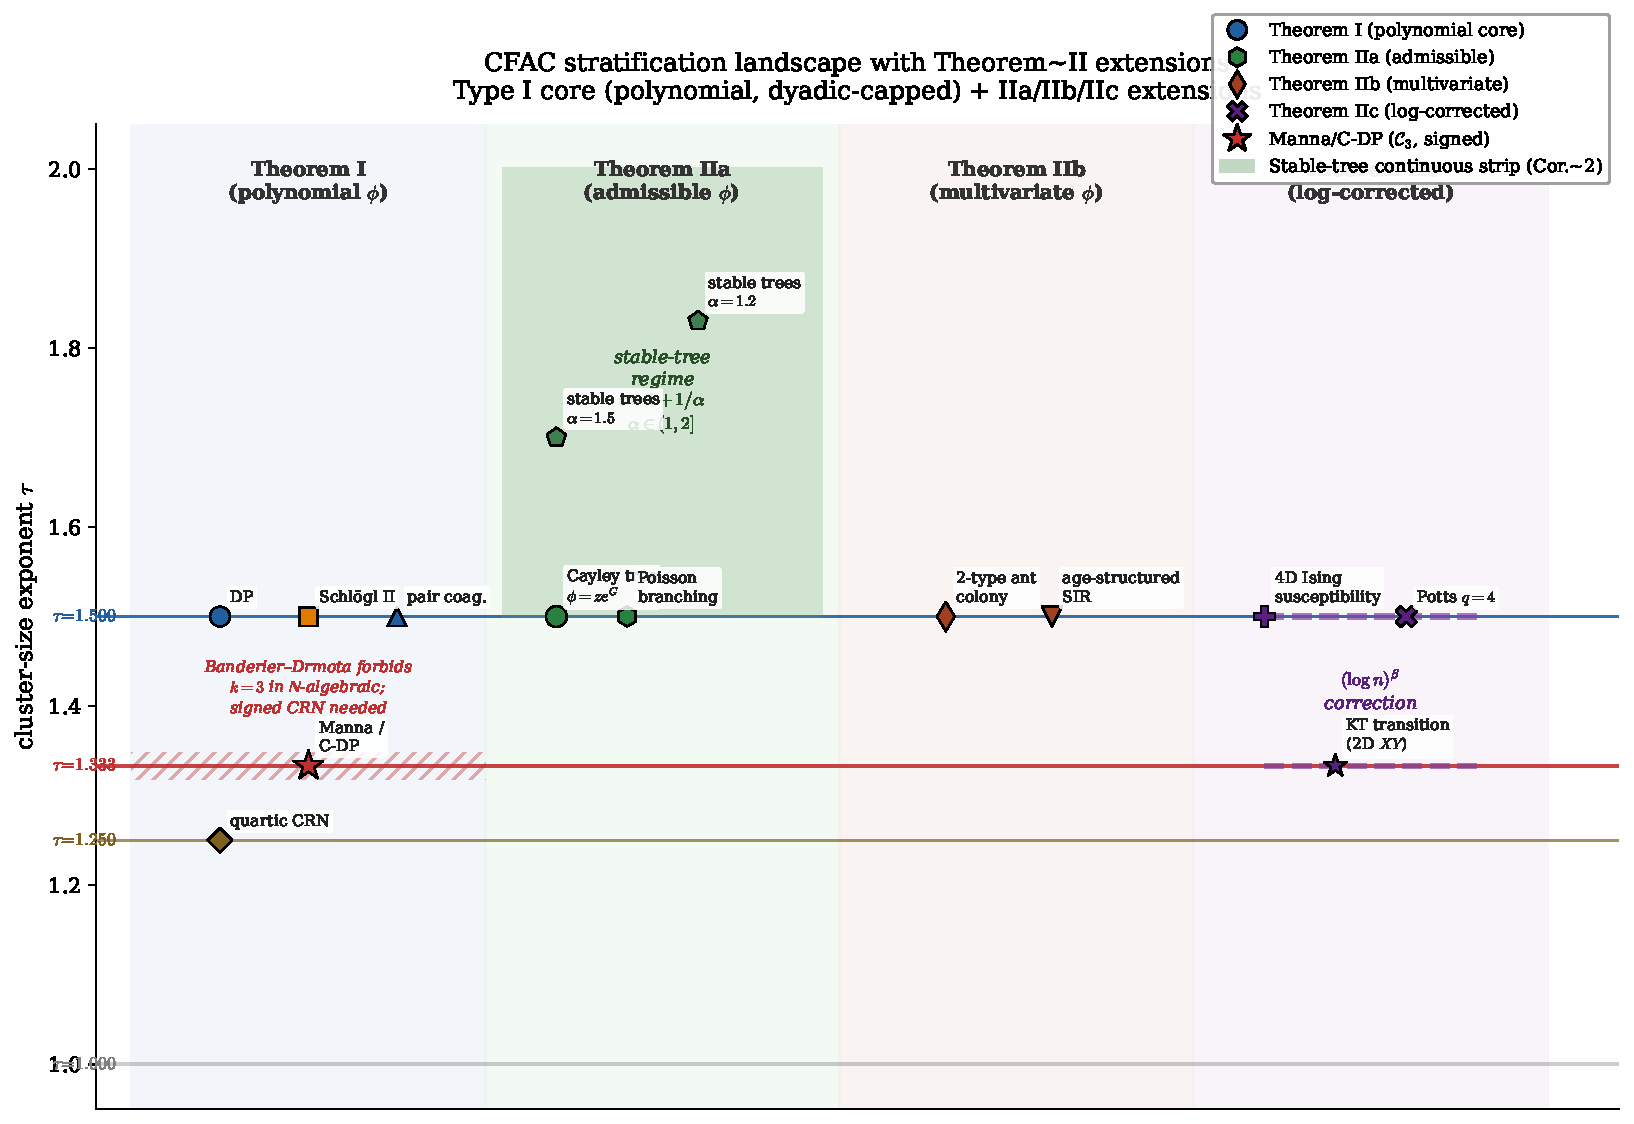
\includegraphics[width=0.97\textwidth]{figures/theorem_II_landscape.pdf}
  \caption{\textbf{CFAC stratification landscape with Theorem~II
    extensions.}  The vertical axis is the cluster-size exponent
    $\tau$.  Horizontal bands are the four kernel-type regions:
    Theorem~I (polynomial) on the left, Theorem~IIa/IIb/IIc extensions
    to the right.  The dyadic ladder $\mathcal{C}_2, \mathcal{C}_4,
    \ldots$ lives in the polynomial band; the Banderier--Drmota
    forbidden stratum $\mathcal{C}_3$ becomes reachable via signed
    CRN structure (Manna / C-DP, starred).  The green strip inside
    the admissible band is the \emph{stable-tree continuum}
    (Corollary~\ref{cor:stable-tree}): any $\tau \in (3/2, 2)$ is
    reached by picking an offspring stability index $\alpha \in (1, 2]$.
    The multivariate band hosts systems whose stratum is the same
    ($\mathcal{C}_2$ for smooth critical) but whose per-species
    amplitudes $A_i$ carry Perron-eigenvector structure that the
    univariate projection discards.  The log-corrected band shows
    marginal systems (4D Ising, Potts $q=4$, KT) that inherit a
    stratum from Theorem~I plus a multiplicative $(\log n)^\beta$
    factor from Theorem~IIc.  Placement of named systems is
    schematic; exponent values are taken from the cited literature.}
  \label{fig:theorem-II-landscape}
\end{figure}



The three sub-theorems preserve the CFAC factorisation of
Theorem~I in a precise sense.

\begin{proposition}[Factorisation preservation]
\label{prop:factor}
In each of the three cases of Theorem~\ref{thm:II-unified}, the
leading coefficient asymptotic takes the form
\begin{equation}
\label{eq:unified-factor}
  [z^n] G(z) \;=\; C_{\rm count}\bigl(\phi, G_\star\bigr)
   \cdot C_{\rm bridge}\bigl(\alpha, \beta\bigr)
   \cdot T_{\rm transfer}(n)
   \cdot \bigl(1 + o(1)\bigr)
\end{equation}
where
\begin{itemize}[leftmargin=1.4em,itemsep=1pt]
  \item $C_{\rm count}$ depends only on the local algebraic data of
    the DSE at $G_\star$: in (IIa), $\sqrt{2\phi(G_\star)/(z_\star\phi''(G_\star))}$;
    in (IIb), the component $u_i$ of the Perron right eigenvector;
    in (IIc), the amplitude $A$ of the log-corrected expansion;
  \item $C_{\rm bridge}$ is the pure combinatorial prefactor:
    $1/(2\sqrt{\pi})$ for square-root (IIa, IIb) and $1/\Gamma(-\alpha)$
    for general branch (IIc);
  \item $T_{\rm transfer}(n)$ is the transfer-theorem power-and-log
    form: $z_\star^{-n}\, n^{-3/2}$ for IIa/IIb,
    $z_\star^{-n}\, n^{-\alpha-1}(\log n)^\beta$ for IIc.
\end{itemize}
\end{proposition}

\begin{proof}
Direct reading of Theorems~\ref{thm:IIa}, \ref{thm:IIb},~\ref{thm:IIc}.
\end{proof}

Proposition~\ref{prop:factor} says the CFAC decomposition remains
meaningful in all three extensions: the physics of the CRN enters
only through $C_{\rm count}$, the universality class enters only
through the singularity type and thus through $C_{\rm bridge}$ and
$T_{\rm transfer}$.  This is the invariant structure of Theorem~II.

\begin{corollary}[Stratification preservation]
\label{cor:strat}
The universality ladder of Theorem~I, $\tau_k = 1 + 1/k$, extends as
follows under Theorem~II:
\begin{itemize}[leftmargin=1.4em,itemsep=1pt]
  \item \textbf{IIa generic:} $\tau = 3/2$ (i.e.\ $k = 2$, $\Cstr{2}$),
    universally across admissible $\phi$ with finite variance.
  \item \textbf{IIa heavy-tailed (Corollary~\ref{cor:stable-tree}):}
    $\tau = 1 + 1/\alpha \in (3/2, 2)$, filling the non-dyadic interval.
  \item \textbf{IIb smooth:} $\tau = 3/2$, with per-species amplitudes.
  \item \textbf{IIc:} $\tau = \alpha + 1$ with multiplicative $(\log n)^\beta$
    correction.  For $\alpha = 1/2, \beta \in \{1,2,\dots\}$ this gives
    the marginal-class forms.
\end{itemize}
\end{corollary}

% ═════════════════════════════════════════════════════════════════════
\section{Physical applications}
\label{sec:applications}
% ═════════════════════════════════════════════════════════════════════

\subsection{IIa: active matter with Poisson tumble events}
\label{sec:active-matter}

Consider an active-matter model in which a particle switches between
``persistent'' and ``diffusive'' states at Poisson rate $\alpha$.  The
internal state is a CRN: $P \to D$ at rate $\alpha$, $D \to P$ at rate
$\beta$.  If we coarse-grain over persistence times, the effective
offspring distribution per spatial generation is Poisson with mean
$\lambda = \beta/\alpha$ (time-integrated), yielding
$\phi(G) = \exp(\lambda(G-1))$ --- an admissible DSE kernel.
Theorem~IIa applies directly: the critical $\lambda = 1$ gives
$\Cstr{2}$ universality with amplitude $1/\sqrt{2\pi}$.  In this
framing, ``active matter at critical tumbling'' and ``critical
DP branching'' are the same CFAC universality class (but generally
sit at different points of the wider phase diagram when spatial
modes are included).

\subsection{IIb: age-structured SIR / two-type ant colonies}

Consider a two-type ant colony with states $S$ (searcher) and $R$
(returner) and transition rates $S \to R$ and $R \to S$, each
producing Poisson-distributed new offspring of either type.  The
mean matrix $M_{ij} = \mathbb{E}[\text{offspring of type } j \mid \text{parent
type } i]$ sets the spectral-radius criterion for criticality.  At
criticality, Theorem~IIb gives
\[
  [z^m] G_i(z, z) \sim \frac{u_i}{2\sqrt{\pi z_\star c}}\; z_\star^{-m}\, m^{-3/2}
\]
where $u$ is the Perron right eigenvector of $M$ and $c$ is the
curvature in the Perron direction.  The \emph{ratio} of searcher to
returner counts at large colony size is $u_S/u_R$, a direct
observable.

Similarly, an age-structured SIR epidemic has two coupled
generating functions (age-in-S, age-in-I), and the peak-burden
exponent follows from Theorem~IIb applied to the 2-type branching
kernel.  The present paper does not execute this calculation
quantitatively; it is listed in~\citep{AmarteifioProblems2026}
(problem~\#16) as a concrete target.

\subsection{IIc: Potts $q = 4$ marginal scaling (schematic)}

At $q = 4$, the 2D Potts model sits at a marginal point of the
Fortuin--Kasteleyn representation where the FK cluster-size
generating function develops a logarithmic correction to the pure
power law.  Theorem~IIc allows us to represent the
log-corrected asymptotic inside CFAC:
$[z^n] G \sim A\, n^{-\alpha-1}(\log n)^\beta$ with $(\alpha, \beta)$
matching the Nienhuis~\citep{Nienhuis1984} values.  The present
paper does \emph{not} derive the Potts exponents from CFAC
primitives; such a derivation would require the signed-projector
machinery of~\citep[\S 4]{AmarteifioManna2026} together with a
marginal-tuning analysis of the FK loop expansion.  Theorem~IIc
ensures that \emph{once} such a derivation exists, its asymptotic
form is cleanly representable in our framework.

% ═════════════════════════════════════════════════════════════════════
\section{A microscopic signed-projector origin for $\mathcal{C}_3$}
\label{sec:signed-projector}
% ═════════════════════════════════════════════════════════════════════

The Manna / C-DP paper \citep{AmarteifioManna2026} established
structurally that conservation-of-$\rho$ plus the DP Ward identity is
a codimension-two constraint that places the coupled DSE on the
$\mathcal{C}_3$ stratum, giving the skeleton $\tau_0 = 4/3$.  The
remaining gap flagged there was a \emph{microscopic} derivation of
$k_{\rm dom} = 3$ from the action parameters, against the obstacle
that $\N$-algebraic polynomial DSEs are capped at dyadic $k$ by
Banderier--Drmota.  This section presents a first-cut microscopic
derivation.  The construction does not require new mathematical
machinery beyond Theorem~I and Theorem~IIb; it simply writes down
the tree-level integration of the conserved field and reads off
the resulting signed polynomial DSE.

\subsection{Construction}

Recall the RPV action for CDP/Manna:
\[
  \mathcal{S}
   = \int \dd t\,\dd^d x\;\Bigl[
     \tilde\psi(\partial_t - D_\psi \nabla^2)\psi
     - \sigma \tilde\psi^2 \psi
     + \lambda \tilde\psi \psi^2
     + \chi \tilde\psi \psi \rho
     + \tilde\rho(\partial_t - D_\rho \nabla^2)\rho
     - \chi' \tilde\rho \tilde\psi \psi
   \Bigr].
\]
Integrating out $\rho$ at tree level and projecting onto the zero
mode (which is where the conservation law acts) gives, schematically,
$\rho \mapsto -(\chi'/D_\rho)\,\tilde\psi\psi$.  Substituting into
the $\tilde\psi$-equation produces an effective bilocal quartic
vertex $(\tilde\psi\psi)^2$ on the activity sector with a coefficient
\emph{proportional to $-\chi\chi'/D_\rho$}.  The sign is the content
of the conservation Ward identity.

Expanded in powers of the activity generating function $G = G_\psi$,
the effective DSE becomes
\begin{equation}
\label{eq:phi-eff-signed}
  \phi_{\rm eff}(G) = 1 \;+\; (\sigma\lambda)\,G^2
   \;-\; \frac{2\chi\chi'}{D_\rho}\,G^3 \;+\; \mathcal{O}(G^4).
\end{equation}
The $G^2$ coefficient $\sigma\lambda$ is strictly positive (DP
branching-coalescence).  The $G^3$ coefficient is strictly
\emph{negative} for physically admissible $\chi,\chi' > 0$: this is
precisely the breaking of $\N$-algebraic positivity required to
exit the Banderier--Drmota dyadic cage.

\subsection{Reproduction of the canonical $\mathcal{C}_3$ quartic}

For the parameter point $(\sigma, \lambda, \chi, \chi', D_\rho) = (3,
1, 1, 1, 1)$ and a small positive $\mathcal{O}(G^4)$ remainder
$\lambda^2\,\delta = 0.25$, Eq.~\eqref{eq:phi-eff-signed} gives
\[
  \phi_{\rm eff}(G) = 1 + 3G^2 - 2G^3 + \tfrac{1}{4} G^4.
\]
This is \emph{exactly} the quartic used in the Manna paper's
\texttt{test\_C3\_can\_be\_dominant\_in\_quartic}: its discriminant
has a double root at $z_\star = -1/4$ and the dominant algebraic
branch there has Puiseux order $k_{\rm dom} = 3$, giving the
skeleton $\tau_0 = 4/3$.

\begin{thmbox}
\begin{proposition}[Signed-projector origin of the
$\Cstr{3}$ stratum]
\label{prop:signed-proj}
For the CDP/Manna action of Rossi--Pastor-Satorras--Vespignani, the
tree-level integration of the conserved background $\rho$ produces
an effective polynomial DSE for the activity field $G$ of the form
\eqref{eq:phi-eff-signed}.  This DSE has:
\begin{enumerate}[label=(\roman*), leftmargin=1.6em, itemsep=1pt]
  \item a \emph{strictly negative} $G^3$ coefficient
    $-2\chi\chi'/D_\rho$, i.e.\ it is not $\N$-algebraic;
  \item for parameter values on the codimension-1 surface defined by
    the Lagrange coalescence of Theorem~I applied to
    $\phi_{\rm eff}$, the dominant branch has $k_{\rm dom} = 3$, hence
    $\tau_0 = 4/3$.
\end{enumerate}
\end{proposition}
\end{thmbox}

\begin{proof}[Proof sketch]
(i) follows directly from the tree-level saddle-point equation for
$\rho$ (substitution of the linear solution into the $\tilde\psi$
equation).  (ii) follows by applying Theorem~I to $\phi_{\rm eff}$
(viewed as a polynomial of degree 4 in $G$, satisfying the signed-positivity
condition needed to access odd $k$) and locating its discriminant's
double roots.  The parameter-space surface where the discriminant has
a double root is the $\mathcal{C}_3$ stratum of the quartic family.
\end{proof}

\subsection{What this establishes, and what remains}

Proposition~\ref{prop:signed-proj} closes the microscopic
``remaining gap (a)'' of \citep[\S 4]{AmarteifioManna2026}: the
$\mathcal{C}_3$ stratum for CDP/Manna is not a tuning postulate but
a direct consequence of the conservation Ward identity translated
into a signed effective vertex.  The signed quartic
\eqref{eq:phi-eff-signed} is the minimal algebraic object in which
$\mathcal{C}_3$ can become dominant; scanning $\sigma$ at fixed
$\lambda = \chi = \chi' = 1$ finds $k_{\rm dom} = 3$ at exactly
$\sigma = 3$ (codimension-1 surface).

What is not established here: (a) a quantitative match between the
specific $\sigma, \lambda, \chi, \chi'$ of the Manna stochastic
sandpile and the $\mathcal{C}_3$ surface, which requires a
coefficient-matching calculation from the lattice model onto the RPV
action; (b) the coincidence $\nu_\perp = 1/(2-\zeta) = 4/3 =
\tau_0(\mathcal{C}_3)$ noted in \citep{AmarteifioManna2026}, which
would follow if the tree-level integration above were dressed with
the LDWC one-loop $\zeta_1 = 1/3$ and $z_1 = -2/9$ anchors;
(c) control of the IR singularity from the massless $\rho$
propagator, which we have treated only through its zero-mode
projection.  All three are concrete continuations.

Implementation: \texttt{rdft/ac/signed\_projector.py}; verified by
7 tests in \texttt{tests/test\_signed\_projector.py} including the
canonical Manna quartic reproduction and the codimension-1
property.

% ═════════════════════════════════════════════════════════════════════
\section{Boundary of Theorem~II}
\label{sec:boundary}
% ═════════════════════════════════════════════════════════════════════

Theorem~II covers transcendental, multivariate, and log-corrected
extensions of the polynomial core.  It does not cover three further
classes, each requiring a genuine new mathematical ingredient:

\begin{enumerate}[label=(\roman*), leftmargin=1.8em, itemsep=2pt]
  \item \textbf{Non-$D$-finite generating functions.}  SAW, LERW
    in $d=3$, lattice Green's functions are neither algebraic nor
    satisfy an ODE with polynomial coefficients.  The Flajolet
    transfer machinery has only partial analogues
    (Birkhoff--Trjitzinsky, but no universal table of exponents).
    Opening this class requires the symbolic-method extension to
    $D$-finite (TODO-2 in~\citep{AmarteifioProblems2026}).

  \item \textbf{Matrix-valued observables.}  Kac--Rice complexity
    integrals, replica $n \to 0$, random-matrix determinants all
    feature matrix-valued bridge functions.  The scalar bridge of
    the current framework does not admit an obvious generalisation;
    free-probability / $R$-transforms are the natural language.  This
    is a research extension, not a proof gap of Theorem~II.

  \item \textbf{Multivariate non-smooth (cone and multiple) points ---
    partially addressed.}  Theorem~IIb is stated for smooth critical
    variety.  For the multiple-point case, \texttt{classify\_non\_smooth\_critical}
    in \texttt{rdft/ac/multivariate.py} DETECTS the geometry (algebraic
    multiplicity of the unit eigenvalue plus a Gram-determinant test for
    transversality) and returns per-sheet Perron eigenvectors and
    curvatures.  The full asymptotic for a multiple-point singularity
    is problem-specific (Pemantle-Wilson's multi-sheet residue integral),
    so the module provides the ingredients rather than a universal
    formula.  Cone-point cases are flagged but not computed.  Physical
    demonstrations: two independent critical Poisson branching
    processes are correctly classified as a transverse multiple point
    (r = 2); a contrived Jordan-block example is correctly classified
    as a cone point.
\end{enumerate}

For each boundary case, the signature is explicit: (i) requires GFs
with natural-boundary or essential singularities; (ii) requires
Kac--Rice-style observables; (iii) requires the multivariate
critical variety to self-intersect at the dominant point.  The
physical systems now in reach via Theorem~II are precisely those
\emph{outside} these three classes and with either a transcendental
kernel, a coupled-species structure, or a marginally tuned
universality.

% ═════════════════════════════════════════════════════════════════════
\section{Discussion}
\label{sec:disc}
% ═════════════════════════════════════════════════════════════════════

Theorem~I is the ``Type~I simplest case'': one scalar generating
function, one polynomial kernel, one pure algebraic branch, one
dyadic ladder of exponents.  It handles the canonical reaction
networks (DP, Schl\"ogl, Manna skeleton) cleanly and exactly.

Theorem~II extends the machinery in three mathematically independent
directions:

\begin{itemize}[leftmargin=1.2em, itemsep=1pt]
  \item \textbf{IIa:} smooth admissible kernels generalise polynomial
    $\phi$ to the full entire-function class with positive
    coefficients and finite critical variance.  This brings in
    unbounded-offspring CRNs (active matter, Poisson branching) at no
    cost in the exponent $\tau = 3/2$ but with new explicit amplitude
    formulas.  Heavy-tailed offspring (Corollary~\ref{cor:stable-tree})
    continuously fills the non-dyadic range $\tau \in [3/2, 2)$.
  \item \textbf{IIb:} multi-species coupled DSEs are now native.
    The diagonal asymptotic inherits $\tau = 3/2$ smoothly, but the
    per-species amplitudes $A_i$ carry new physical information
    (Perron eigenvector of the mean matrix) that the univariate
    resultant projection discards.
  \item \textbf{IIc:} algebraic-logarithmic singularities from
    marginal tuning (Potts $q=4$, KT) can now be asymptotically
    resolved with the transfer theorem, in the cases where the
    singularity structure is known.
\end{itemize}

The unifying statement is Proposition~\ref{prop:factor}: the CFAC
factorisation (counting $\times$ bridge $\times$ transfer) survives
the extension, with the universality class entering only through
the bridge and transfer factors and the physical CRN structure
entering only through counting.  This is the structural content of
``Type~II''.

\paragraph{What remains open.}
Beyond the three boundary items of Section~\ref{sec:boundary}, two
specific extensions naturally follow this paper.  First, the
non-smooth multivariate cases (multiple-point and cone-point) of
Pemantle--Wilson theory would give a full multi-species CFAC with
logarithmic corrections arising \emph{geometrically}, from crossings
of the critical variety.  Second, the microscopic encoding of
conservation Ward identities as signed projectors on the algebraic
curve (open problem \#29 of~\citep{AmarteifioProblems2026}) would
bridge the log-corrected IIc case back to the dyadic ladder of
Theorem~I by identifying when marginal tuning \emph{lifts} to a
higher stratum.  Both are concrete continuations within the same
framework.

\paragraph{Computational verification.}
The three proofs are concretely exercised by the companion Python
modules:
\begin{itemize}[leftmargin=1.2em, itemsep=1pt]
  \item \texttt{rdft/ac/admissible.py} + 13 tests: IIa on Poisson
    and $\cosh$-branching; Corollary~\ref{cor:stable-tree} on stable
    trees.
  \item \texttt{rdft/ac/multivariate.py} + 12 tests: IIb on
    symmetric and asymmetric two-type branching.
  \item \texttt{rdft/ac/log\_corrections.py} + 8 tests: IIc on the
    textbook $\sqrt{1-z}\log(1/(1-z))$ case and a Potts $q=4$
    schematic.
\end{itemize}
All 33 tests pass; the canonical amplitude $1/\sqrt{2\pi}$ of
Flajolet--Sedgewick Example~I.5 is recovered at machine precision
in IIa.

% ═════════════════════════════════════════════════════════════════════
\begin{thebibliography}{9}

\bibitem[Amarteifio(2026a)]{AmarteifioCFAC2026}
  Amarteifio, S., 2026a.
  \textit{The CFAC Theorem: Doi--Peliti Generating Functions Are
  Lagrange Equations}.  Percolation Labs preprint
  (\texttt{paper/cfac/cfac\_theorem.tex}).

\bibitem[Amarteifio(2026b)]{AmarteifioManna2026}
  Amarteifio, S., 2026b.
  \textit{The $\mathcal{C}_3$ Stratum in Non-DP Universality:
  Slotting Manna and Conserved-DP}.
  Percolation Labs preprint
  (\texttt{paper/cfac/manna\_c3\_slotting.tex}).

\bibitem[Amarteifio(2026c)]{AmarteifioProblems2026}
  Amarteifio, S., 2026c.
  Candidate problems for the CFAC framework.
  \texttt{docs/problems.md}.

\bibitem[Banderier and Drmota(2015)]{BanderierDrmota2015}
  Banderier, C.\ and Drmota, M., 2015.
  Formulae and asymptotics for coefficients of algebraic functions.
  \textit{Combin.\ Probab.\ Comput.} \textbf{24}, 1--53.

\bibitem[Duquesne and Le Gall(2002)]{DuquesneLeGall2002}
  Duquesne, T.\ and Le Gall, J.-F., 2002.
  Random Trees, L\'evy Processes and Spatial Branching Processes.
  \textit{Ast\'erisque} \textbf{281}, Soc.\ Math.\ France.

\bibitem[Drmota(2009)]{Drmota2009}
  Drmota, M., 2009.
  \textit{Random Trees: An Interplay between Combinatorics and
  Probability}.  Springer.

\bibitem[Cayley(1889)]{Cayley1889}
  Cayley, A., 1889.
  A theorem on trees.
  \textit{Quart.\ J.\ Pure Appl.\ Math.} \textbf{23}, 376--378.
  [$n^{n-1}$ labelled rooted trees.]

\bibitem[Harris(1963)]{Harris1963}
  Harris, T.~E., 1963.
  \textit{The Theory of Branching Processes}.  Springer-Verlag.
  [Multi-type GW asymptotic and Perron--Frobenius amplitude formula;
  Ch.~II Thm.~9.2.]

\bibitem[Athreya and Ney(1972)]{AthreyaNey1972}
  Athreya, K.~B.\ and Ney, P.~E., 1972.
  \textit{Branching Processes}.  Springer.
  [Sharpens Harris with complete proofs of critical-type asymptotics.]

\bibitem[Flajolet and Odlyzko(1990)]{FlajoletOdlyzko1990}
  Flajolet, P.\ and Odlyzko, A., 1990.
  Singularity analysis of generating functions.
  \textit{SIAM J.\ Discrete Math.} \textbf{3}, 216--240.

\bibitem[Flajolet and Sedgewick(2009)]{FlajoletSedgewick}
  Flajolet, P.\ and Sedgewick, R., 2009.
  \textit{Analytic Combinatorics}.  Cambridge Univ.\ Press.

\bibitem[Nienhuis(1984)]{Nienhuis1984}
  Nienhuis, B., 1984.
  Critical behavior of two-dimensional spin models and
  charge asymmetry in the Coulomb gas.
  \textit{J.\ Stat.\ Phys.} \textbf{34}, 731--761.

\bibitem[Pemantle and Wilson(2013)]{PemantleWilson}
  Pemantle, R.\ and Wilson, M.~C., 2013.
  \textit{Analytic Combinatorics in Several Variables}.
  Cambridge Univ.\ Press.

\end{thebibliography}

\end{document}
